\documentclass[14pt]{mmcs-article}
\usepackage[russian]{babel}
\usepackage{amsmath, amsthm, amsfonts, amssymb}

\graphicspath{{images/}}

\begin{document}

\section*{Введение}

\textbf{Определение 1.}

\textsl{Двудольным графом} будем называть тройку $\langle V,E,f \rangle$, такую, что:

\begin{itemize}
    \item $V = A \cup B$ и $A \cap B = \emptyset$;
    \item $f: E \rightarrow A \times B$;
\end{itemize}

Где $V$ ~--- множество вершин, разбитое на два непересекающихся подмножества $A$ и $B$.
$E$ ~--- множество дуг.
$f$ ~--- отображение, ставящее в соответствие каждой дуге упорядоченную пару вершин.

\textbf{Определение 2.}

\textsl{Обхватом графа} называют длину его минимального цикла.

\textbf{Замечание 1.}

Отметим, что обхват любого двудольного графа является чётным числом, большим, чем два.

\textbf{Замечание 2.}

Известно, что на практике для кодирования эффективнее использовать графы с большим обхватом.

\pagebreak
\section*{Метаграфы}

\textbf{Определение 3.}

\textsl{Метаграфом} будем называть четвёрку $\langle A \cup B,E,f,w \rangle$, такую, что:

\begin{itemize}
    \item $\langle A \cup B,E,f \rangle$ ~--- двудольный граф;
    \item $w: E \rightarrow \mathbb{Z}$ ~--- отображение задающее веса дуг.
\end{itemize}

На (рис. \ref{image:2}) представлен пример метаграфа с тремя вершинами и четырьмя дугами.

\begin{figure}[H]
    \centering
    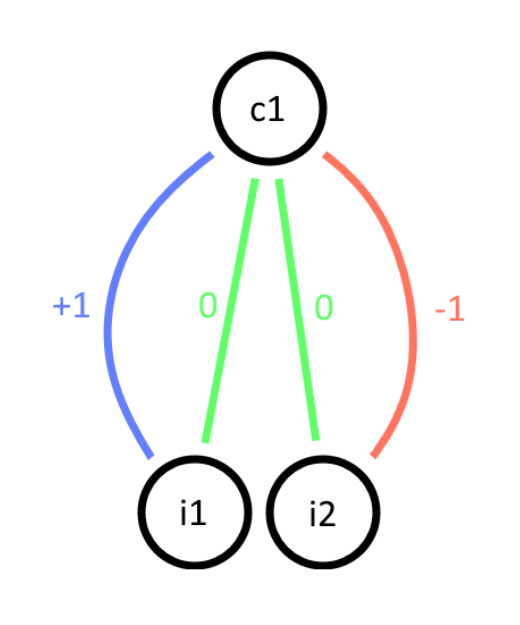
\includegraphics[scale=0.4]{Fig_2.png}
    \caption{ Метаграф с весами дуг +1, 0, 0, -1.. }
    \label{image:2}
\end{figure}

Пусть $G$ ~--- метаграф, $G = \langle A \cup B,E,f,w \rangle$, и задано число $r \in \mathbb{N}$. Построим двудольный граф $G^{(r)} = \langle A' \cup B',E',f' \rangle$ по следующим правилам:

\begin{itemize}
    \item $V^{(r)} = \{ v^{(j)} \}_{v \in V, j = 1..r}$,
    будем говорить , что вершины $v^{(j)}$ на графе G соответствуют вершине $v$ на графе $G^{(r)}$ и наоборот;
    \item $E^{(r)} = \{ e^{(j)} \}_{e \in E, j = 1..r}$,
    будем говорить , что дуги $e^{(j)}$ на графе G соответствуют дуге $e$ на графе $G^{(r)}$ и наоборот;
    \item $f^{(r)}(e^{(j)}) = ([first(f(e))]^{(j)}, [second(f(e))]^{(j + w(e) (mod \ r))})$.
\end{itemize}

\textbf{Определение 4.}

Граф $G^{(r)}$, построенный в ходе работы Алгоритма 1. будем называть расширением метаграфа $G$ в $r$ раз.

На (рис. \ref{image:3}) изображён граф, полученный расширением метаграфа из (рис. \ref{image:2}) в 4 раза.

\begin{figure}[H]
    \centering
    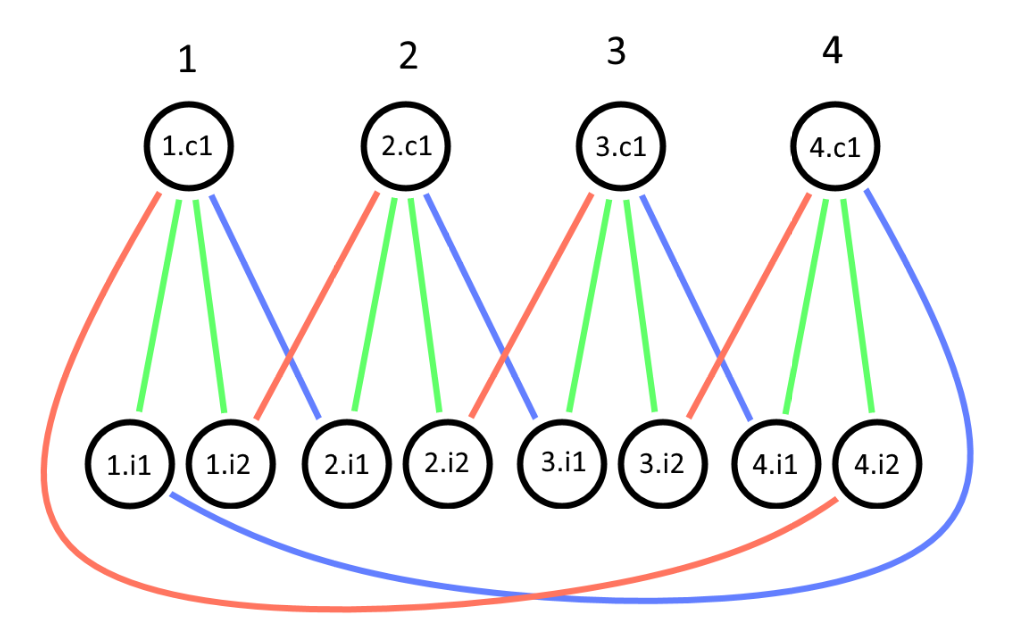
\includegraphics[scale=0.4]{Fig_1.png}
    \caption{ Метаграф с весами дуг +1, 0, 0, -1.. }
    \label{image:3}
\end{figure}

\textbf{Определение 5.}

Введём вспомогательные функции для работы с парами:

$first: X \times Y \rightarrow X: first(x, y) = x;$

$second: X \times Y \rightarrow Y: second(x, y) = y;$

\textbf{Определение 6.}

Введём обозначение для множества вершин или дуг, порождаемых из одной вершины или дуги в процессе расширения метаграфа:

$T^{(r)}_v = \{ v^{(i)} \}_{i=1}^r \forall v \in V \cup E.$

% \textbf{Определение 7.}

% Пусть $G = \langle V, E, f, w \rangle$ ~--- метаграф. $j$-той компонентой будем называть множество вершин $\{ v^{(j)} \}_{v \in V}$.

\textbf{Теорема 1.}

Если на метаграфе $G$ есть путь $\phi = (e_1, ..., e_{\ae})$, то на графе $G^{(r)}$ есть попарно не пересекающиеся пути $\psi_j = (e^{(x_{j, 1})}_1, ..., e^{(x_{j, \ae})}_{\ae})\forall x_{j, 1} = j, j \in 1..r$, причём $e^{x_{j, i}}_i \in T^{(r)}_{e_i}$.

\textbf{Доказательство.}

Следует из определения расширения метаграфа.

\qed

\textbf{Определение}

Такие пути будем называть соответстующими

\textbf{Замечание 2.}

Из того, что на метаграфе есть цикл не следует, что цикл есть на расширенном графе.

$/*$ Надо добавить пример, сейчас он есть только на бумажечке $*/$

\pagebreak

\textbf{Определение 7.}

Пусть $G = \langle V, E, f, w \rangle$ ~--- метаграф. Характеристикой пути $\phi = (e_1, ..., e_{\ae})$ будем называть

\[
    ch(\phi) = \sum_{i = 1}^{\ae}(-1)^{i - 1}w(e_i).
\]

\textbf{Теорема 2.}

Пусть дан метаграф $G$. На нём задан путь $\phi = (e_1, ..., e_{\ae})$. на расширенном графе ему соответствуют пути $\psi_l = (e'_1, ..., e'_{\ae})$.

Пусть первая вершина в пути ~--- $\psi_l = v_f^{(j)}$, тогда последняя вершина этого пути ~--- $\psi_l = v_e^{(j + ch(\phi))}$.

\textbf{Доказательство.}

$/*$ Тт у меня пока не хватило сил переписать, но я перепишу $/*$

Первая вершина цикла $\phi$ ~--- $v_1 = first(f(e_1))$, тогда первая вершина пути $\psi$, $v'_1 = v_1^{(1)}$.

Вторая вершина цикла $\phi$ ~--- $v_2 = second(f(e_1))$, тогда вторая вершина пути $\psi$, $v'_2 = v_1^{(1 + w(e_1))} = v_1^{1 + ch(e_1)}$.

$(2i + 1)$-вая вершина цикла $\phi$ ~--- $v_{2i + 1} = first(f(e_{2i}))$, $(2i + 1)$-вая вершина цикла $\psi$ ~--- $v'_{2i + 1} = v_{2i + 1}^{(1 + w(e_1) - w(e_2) + ... - w(e_{2i}))} =  v_{2i + 1}^{1 + ch(e_1, e_2, ..., e_{2i})}$.

Последняя вершина цикла $\phi$ ~--- $v_{\ae + 1} = first(f(e_{\ae}))$, последняя вершина цикла $\psi$ ~--- $v'_{\ae + 1} = v_{2i + 1}^{(1 + ch(e_1, e_2, ..., e_{\ae}))} = v_{2i + 1}^{(1 + ch(\phi))}$

$ch(\phi) = 0$ тогда и только тогда, когда первая и последняя вершины пути совпали, то есть он является циклом.

\qed

\textbf{Следствие.}

Пусть $\phi$ ~--- цикл на метаграфе. Тогда соответствующие ему пути на расширенном графе являются цциклоами тогда и только тогда, когда $ch(\phi) = 0$.

$/*$ Надо добавить пример, сейчас он есть только на бумажечке $*/$

\textbf{Алгоритм 1.}

Поиска цикла с длинной меньше или раной заданному числу $l \in \mathbb{N}$.

Пусть $G = \langle A \cup B, E,f,w\rangle$ ~--- метаграф. Для каждой вершины $a \in A:$

\begin{itemize}
    \item Пометим $a$ парой $(0, 0)$.
    \item В цикле по поколениям $g$ от $1$ до $l$:
      \begin{itemize}
      \item Для всех меток $label = (ch, g - 1)$:
        \begin{itemize}
        \item Вершину, которая помечена меткой $label$, обозначим $v$.
        \item Для всех дуг $e: v \in f(e)$:
          \begin{itemize}
          \item $ch' = ch + (-1)^{g} w(e)$
          \item Обозначим $v'$ вершину, такую, что $v' \in f(e), v' \neq v$.
          \item Если $v'$ ещё не была помечена меткой $(ch', g') \forall g'$ ~--- пометим её парой $(ch', g)$.
          \item Если $v'$ помечена помечена парой $(ch', g)$ ~--- сообщаем о том, что найден цикл длины $g * 2$ и завершаем работу алгоритма.
          \end{itemize}
        \end{itemize}
      \end{itemize}
    \item Сообщаем о том, что цикл не найден и завершаем работу алгоритма.
\end{itemize}

\pagebreak
\section*{Построение графов с заданным обхватом}

$/*$ Слова о задаче. $*/$

\textbf{Теорема 3.}

Пусть $l \in \mathbb{N}.$ И задан метаграф $G = <V, E, f, w>$, причём $w(e_i) = x_i \forall i = 0..|E|$.

Сотставим систему неравенств, содержащую все неравенства вида $ch(\phi) \neq ch(\psi) : a \in A, v \in V, \phi, \psi$ ~--- пути из $a$ в $v$ равной длины $\leq l$.

Её решение даёт метаграф, расширение которого имеет обхват не меньше $2l$. Если решения нет, значит не существует расширения метаграфа $G$ c обхватом меньше или равным $2l$.

\textbf{Доказательство.}

Пусть в полученном расширенном графе обнаружен цикл длины $t < 2l$. Тогда есть цикл $\phi = (e_1, ..., e_{\ae})$ на метаграфе, характеристика которого равна нулю.

Разделим цикл на два пути $(e_1, ..., e_{\ae/2})$ и ${e_{\ae}, ..., e_{\ae/2 + 1}}$. Пути имеют одинаковую длину $t / 2$ и одинаковую характеристику по модулю $r$, что противоречит условию теоремы.

\qed


\end{document}